\subsection{Speed analysis}
In this section, we investigate the average speed $\overline{speed}$ in each status. For example, taxi i drives in occupied status for a distance $d$ using time $t$, then the average speed in this status is $d/t$.
From March 3th to 7th, 2011, the $\overline{speed_{empty}} = 3.627 m/s$, while that for occupied status is $\overline{speed_{occupied}}=7.083 m/s$. 

\begin{figure}
\centering
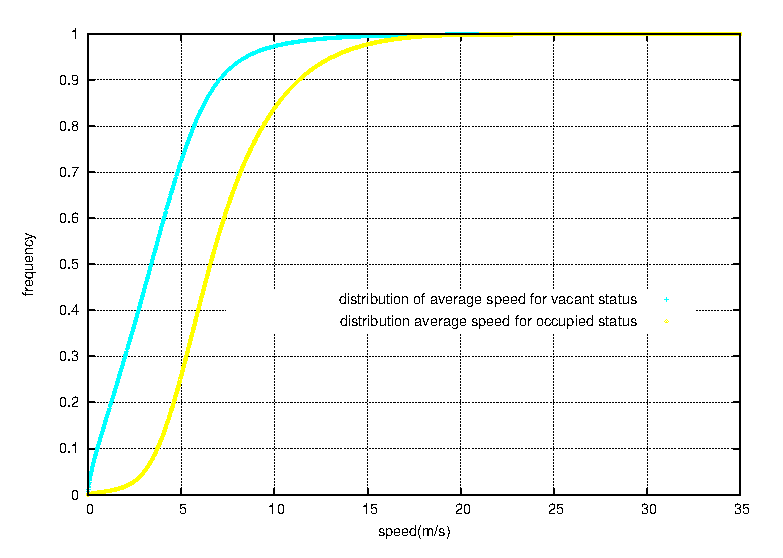
\includegraphics[width=0.4\textwidth]{figures_201103/assumption/speeddis.eps}
\caption{Speed Distribution for vacant and occupied status.}\label{figure_speed_distribution}
\end{figure}

To further investigate the speed distribution, proportion for every $\overline{speed}$ section is calculated, in fig.\ref{figure_speed_distribution}. For example, dot(x,y) means $2.45\%$ records fall in the speed range $[0,20)km/h$.
Fig. \ref{figure_speed_distribution} shows that $\overline{speed}$ distribution differs for each status. For vacant status, the $\overline{speed}$ gather together at  \ref{figure_speed_distribution} also demonstrates that the speed distribution is with strong regularity for each status.


